% Section content template for individual Educative lessons
% This file contains the actual content for a specific section
% Generated from Educative API section content

% Section: System Design: The Pub-Sub Abstraction
% Section ID: 4996814243889152
% Section Slug: system-design-the-pub-sub-abstraction
% Generated: 2025-12-07T21:16:31.799636

\subsection{What is a pub-sub system?}\label{CCKHCe-WJiwyrcMfnyazm}
\\
\textbf{Publish-subscribe messaging}, often known as \textbf{pub-sub messaging}, is an asynchronous service-to-service communication method that's popular in serverless and microservices architectures. Messages can be sent asynchronously to different subsystems of a system using the pub-sub system. All the services subscribed to the pub-sub model receive the message that's pushed into the system.
\\
For example, when a famous athlete posts on Instagram or shares a tweet, all of their followers are updated. Here , the athlete is the publisher, their post or tweet is the message, and all of their followers are subscribers.

\begin{figure}[htbp]
 \centering
 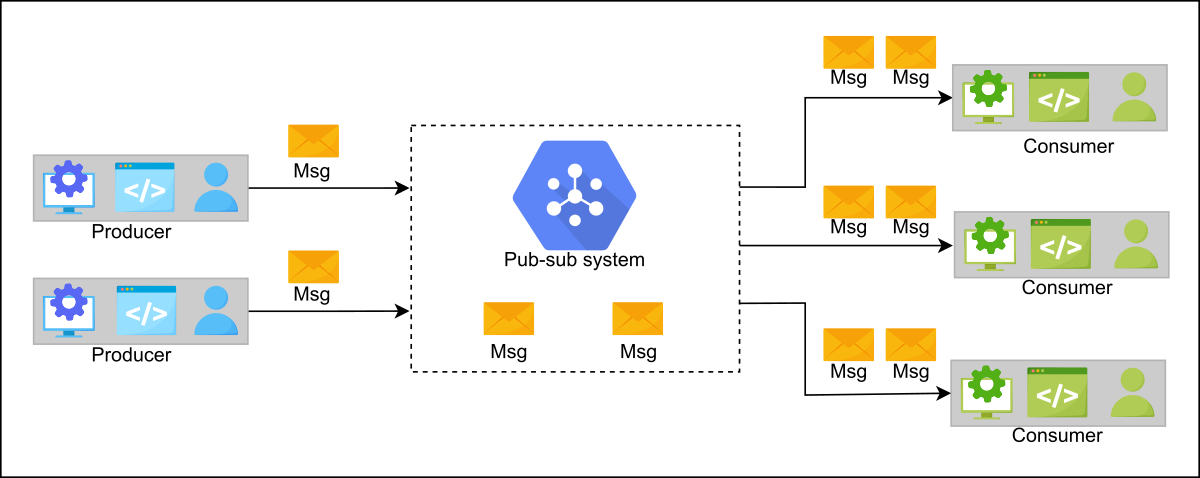
\includegraphics[width=0.5\textwidth]{Images/chapter_18/section_4996814243889152/4981835279237120.png}
 \caption{The pub-sub system}
\end{figure}

\subsection{Motivation}\label{Tk7LsOtTx3O7YX5e2TiDc}
\\
The hardware infrastructure of distributed systems consists of millions of machines. Using a pub-sub system to communicate asynchronously increases scalability. Producers and consumers are disconnected and operate independently, thereby allowing us to scale and develop them separately. The decoupling between components, producers and consumers, allows greater scalability because adding or removing any component doesn't affect the other components.

\subsection{How do we design a pub-sub system?}\label{OWCvPqO8t4uUcHd3o8kVy}
\\
We have divided the pub-sub system design into the following lessons:

\begin{enumerate}
\item
\protect\phantomsection\label{DQI2WdVshHigKU6LurAv_}
\href{https://www.educative.io/courses/grokking-the-system-design-interview/introduction-to-pub-sub}{\textbf{Introduction}}: In this lesson, we learn about the use cases of the pub-sub system, define its requirements, and design the API for it.
\item
\protect\phantomsection\label{z3p_EHd-Vpc_Y_7oMLWmb}
\href{https://www.educative.io/courses/grokking-the-system-design-interview/design-of-a-pub-sub-system}{\textbf{Design}}: In this lesson, we discuss two designs of the pub-sub system, one with messaging queues and the other with a broker.
\end{enumerate}

% End of section content